% Source: tex/chapters/ch06/07_ソフトウェアエンジニアリング運用制御.tex
\subsubsection{監視、測定、追跡、レビュー}

運用では、容量、継続性、可用性を監視する。DevOpsの考え方では、希望的観測に頼ってはならない。システム品質と運用状態を、証拠に基づいて判断する必要がある。

\par\smallskip\noindent\refstepcounter{table}\label{tab:ch06-07}\textbf{表 \thetable: 第06章 ソフトウェアエンジニアリング運用 表07}\par\smallskip
\begin{longtable}{L{55mm}L{95mm}}
\toprule
測定対象 & 意味 \\
\midrule
本番システム監視と製品テレメトリ & 本番で何が起きているかを示す。ログ、トレース、利用者行動、資源使用量などを含む。 \\
リリース前後の検証結果 & リリースが期待どおりに動くか、リリース後に品質が悪化していないかを示す。 \\
利用者活動と資源使用 & どの機能が使われ、どの資源が消費されているかを示す。 \\
影響分析結果 & ある変更がどの機能、構成、利用者に影響するかを示す。 \\
依存関係 & サービス運用に必要な内部依存と外部依存を示す。 \\
構成変更 & 承認済み配備以外の設定変更や環境差分を検出する。 \\
セキュリティと耐障害性 & 攻撃、障害、復旧に対する能力を示す。 \\
\bottomrule
\end{longtable}

\begin{figure}[htbp]
\centering
\IfFileExists{assets/fig-ch06-09.png}{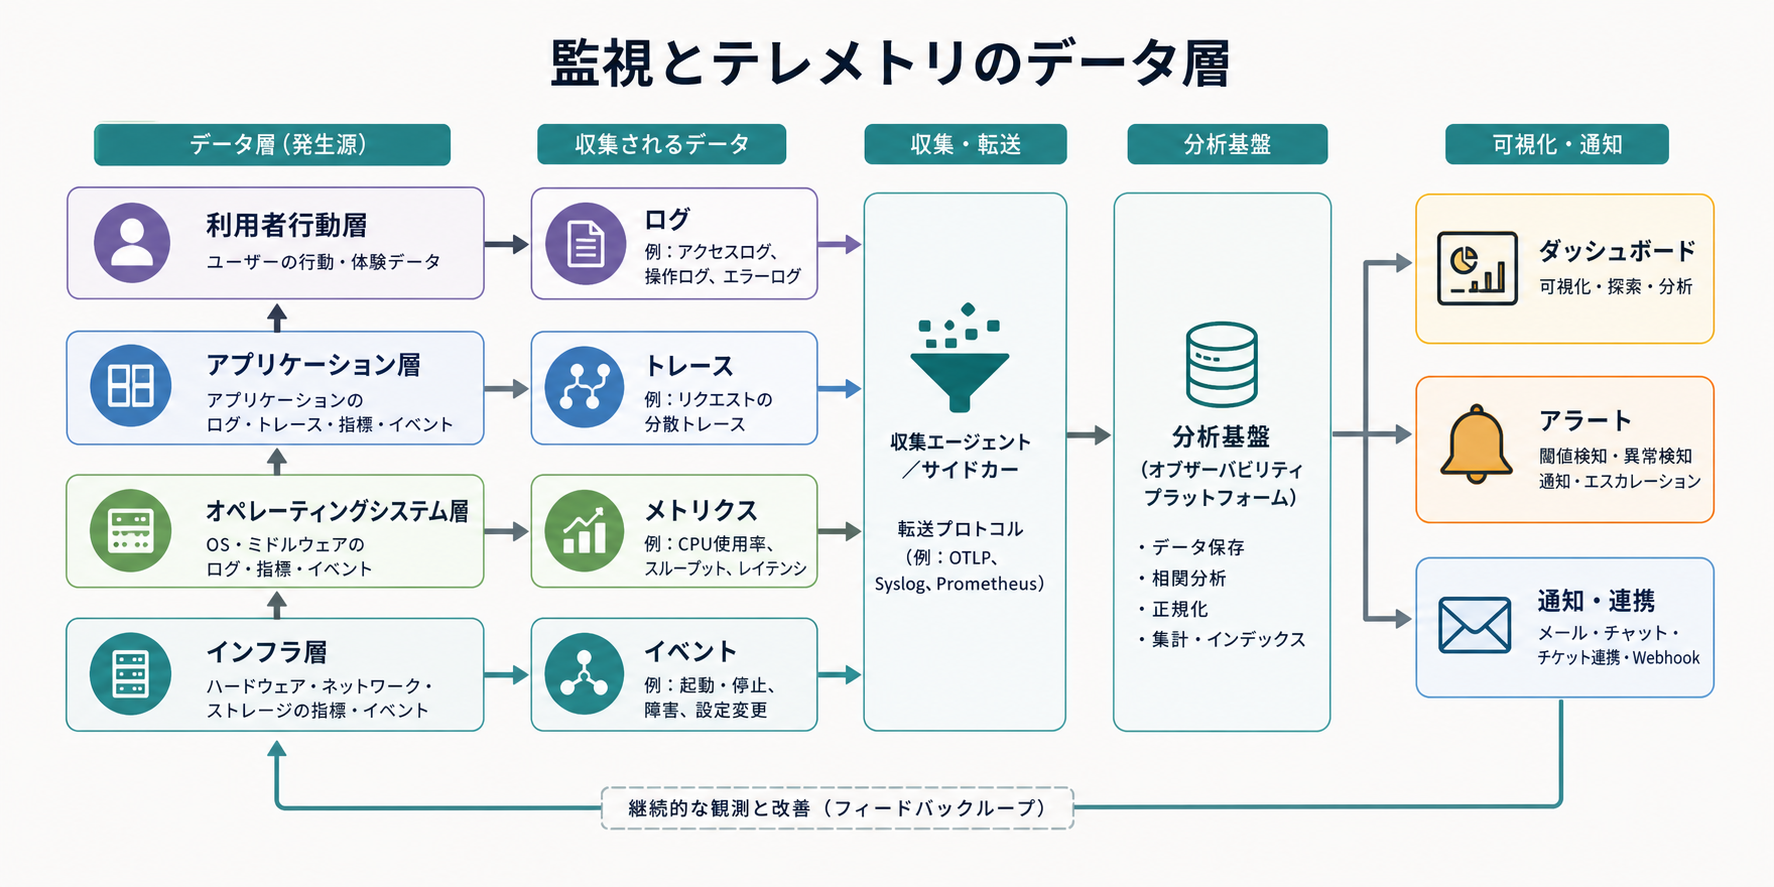
\includegraphics[width=0.96\linewidth]{assets/fig-ch06-09.png}}{\fbox{\parbox[c][48mm][c]{0.9\linewidth}{\centering 画像生成待ち\\監視とテレメトリのデータ層}}}
\caption{監視とテレメトリのデータ層}
\label{fig:ch06-09}
\end{figure}
